\section{Synthetic validation with known flux errors}
\label{sec:synthetic-torque}
The torque experiment uses a known saturated potential with dimensional
bases $I_*=\SI{100}{\ampere}$ and $\psi_*=\SI{0.1}{\weber}$, and $p=3$.
For $x=i_d/I_*$, $y=i_q/I_*$, set $W'=\psi_*I_*\bar W'$ with
\begin{equation}
 \bar W'=x+0.3x^2+0.5y^2-0.01x^4-0.02y^4-0.03x^2y^2+0.02xy^2.
\end{equation}
Its gradient defines the true flux. The synthetic configuration is one
amplitude-invariant three-phase system, so $k_T=3p/2=4.5$.
The ground truth is known; this is separate from the unqualified CAN comparison.
At $I_s=\SI{100}{\ampere}$ add a radial error of \SI{8}{\milli\weber},
a normal error $5\sin(2\theta)$ mWb, or their sum.
\Cref{fig:torque-synthetic} shows that radial error is invisible and that
the mixed residual reproduces only the normal term. Minimum-change torque
agreement would remove that term while retaining the radial error.
The noise panel uses independent zero-mean torque noise with standard
deviation \SI{0.2}{\newton\metre}; its conversion follows the inverse-current
law, not an observed real sensor uncertainty.

\begin{figure}[htbp]
 \centering
 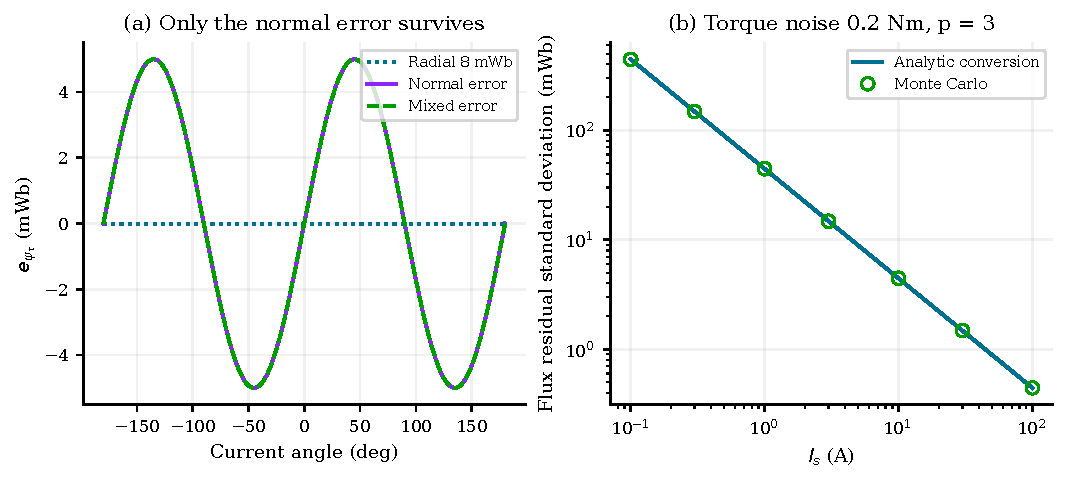
\includegraphics[width=\textwidth]{figures/07_torque_synthetic.pdf}
 \caption{Known-field numerical tests. Left: normal and mixed perturbations
 give the same normalized torque residual; a radial perturbation gives zero.
 Right: the original Monte Carlo noise checks agree with analytic
 $1/I_s$ amplification. Line patterns and open markers distinguish cases.}
 \label{fig:torque-synthetic}
\end{figure}

To test the interaction with reciprocity, use the dimensionless even
potential basis $[1,x,s,(x^2-y^2)/2,s^2]$, with
$x=i_d/I_*$, $y=i_q/I_*$, and $s=(x^2+y^2)/2$ on a full square grid.
Every candidate is reciprocal and has the required reflection.
Torque still annihilates the constant, $s$, and $s^2$ columns.
\Cref{tab:torque-rank} reports the generated ranks: voltage with known
resistance observes both radial slopes, and only the potential gauge remains.
Rows are dimensionless and scaled by $k_{\rm T}I_*\psi_*$ for torque and
$\omega_e\psi_*$ for voltage. These exact rank statements do not require
assuming equal real measurement uncertainties. Narrower current support
can lower rank further.

\begin{table}[htbp]
 \centering
 \begin{tabular}{lrr}
\toprule
Observation block & Rank & Nullity\\
\midrule
Torque & 2 & 3\\
Torque + voltage & 4 & 1\\
Torque + voltage + gauge & 5 & 0\\
\bottomrule
\end{tabular}

 \caption{Generated observation ranks for the five-column reciprocal,
 even potential example. Torque alone leaves two radial modes besides
 gauge; fixing gauge alone would not recover them.}
 \label{tab:torque-rank}
\end{table}

The original forty torque checks are retained, including weighted projection,
rotation, current noise, torque offset/gain, loss terms, resistance signs,
and joint rank. Additional tests cover both current axes, all quadrants,
both torque signs, the origin and small currents, reciprocal positive
isotropic inductance, the even-potential ranks, and excitation slices.
The pointwise projection is also checked to need not preserve conservation.
These are mathematical and implementation checks; no real-map correction
accuracy follows.
